\begin{figure}[!h]
	\centering
	\subbottom[\label{fig:egbui0}]
		{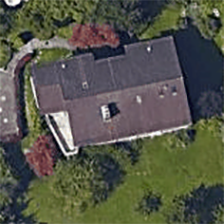
\includegraphics[width=0.243\textwidth]{4-02-0.png}}
	\subbottom[\label{fig:egbui1}]
		{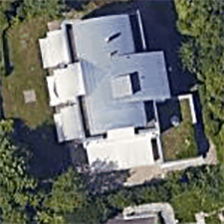
\includegraphics[width=0.243\textwidth]{4-02-1.png}}
	\subbottom[\label{fig:egbui2}]
		{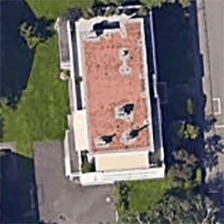
\includegraphics[width=0.243\textwidth]{4-02-2.png}}
	\subbottom[\label{fig:egbui3}]
		{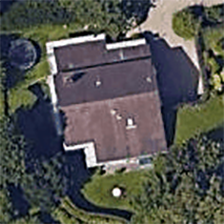
\includegraphics[width=0.243\textwidth]{4-02-3.png}}
	\subbottom[\label{fig:egbui4}]
		{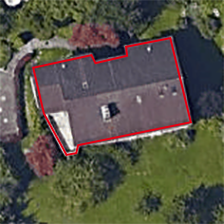
\includegraphics[width=0.243\textwidth]{4-02-4.png}}
	\subbottom[\label{fig:egbui5}]
		{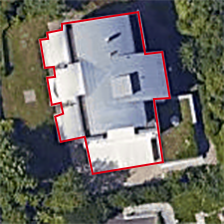
\includegraphics[width=0.243\textwidth]{4-02-5.png}}
	\subbottom[\label{fig:egbui6}]
		{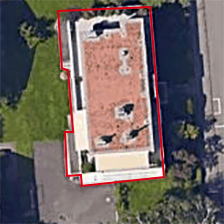
\includegraphics[width=0.243\textwidth]{4-02-6.png}}
	\subbottom[\label{fig:egbui7}]
		{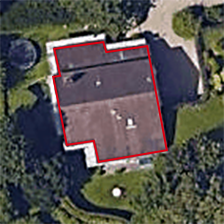
\includegraphics[width=0.243\textwidth]{4-02-7.png}}
    \caption{Example buildings in Zurich for training PolygonRNN. (a)--(d) are the original satellite images obtained by Google Static Maps API. (e)--(g) are (a)--(d) covered by the corresponding polygons' edges, which are visualized based on the ground truth.}
	\label{fig:egbui}
\end{figure}